\chapter{第五单元}

\Needspace{12\baselineskip}

\section{第五单元素养评价（A）}

\Needspace{8\baselineskip}

\pdfbookmark[2]{原书第33页}{orig-33}

\subsection*{原书第33页}

% p033_s01
\BookQuestion{一、1（锐角）}
一个三角形中最少有（\hspace{1.8em}）个锐角。\par
\begin{BookAnswer}
填2。三角形内角和180度，若有两个角都不小于90度，第三角就不可能大于0度。因此每个三角形至少有两个锐角。
\end{BookAnswer}

% p033_s02
\BookQuestion{一、1（钝角）}
一个三角形中最多有（\hspace{1.8em}）个钝角。\par
\begin{BookAnswer}
填1。一个钝角已大于90度，不可能再有第二个钝角；如100度、40度、40度的三角形有1个钝角。
\end{BookAnswer}

% p033_s03
\BookQuestion{一、2（内角和）}
三角形的内角和是（\hspace{1.8em}）。\par
\begin{BookAnswer}
填\(180^\circ\)。任何三角形的三个内角加起来都等于180度。
\end{BookAnswer}

% p033_s04
\BookQuestion{一、2（三边关系）}
三角形任意两边长度的和（\hspace{1.8em}）第三边。\par
\begin{BookAnswer}
填“大于”。三角形任意两边长度之和严格大于第三边；两边之和等于第三边时只能排成一条线。
\end{BookAnswer}

% p033_s05
\BookQuestion{一、3}
有一条腰垂直于梯形的上下两底，这样的梯形叫作（\hspace{1.8em}）。\par
\begin{BookAnswer}
填“直角梯形”。梯形两底平行，一腰垂直两底，就有两个直角。
\end{BookAnswer}

% p033_s06
\BookQuestion{一、4}
在一个长方形中画一条线段，将长方形分成两个梯形，每个梯形都是（\hspace{1.8em}）梯形。\par
\begin{BookAnswer}
填“直角”。切开后每个梯形都保留长方形的两个相邻直角，所以都为直角梯形。
\end{BookAnswer}

% p033_s07
\BookQuestion{一、5（三角形）}
下图中，三角形的高所对应的底边长是（\hspace{1.8em}）厘米。\par
\BookFigure{figures/p033_s07-01.tex}
\begin{BookAnswer}
填6厘米。虚线高8厘米与标有6厘米的边垂直，因此这条高对应的底是6厘米那条边，不是水平的9厘米边。
\end{BookAnswer}

% p033_s08
\BookQuestion{一、5（平行四边形）}
下图中，平行四边形\(AB\)边对应的高是（\hspace{1.8em}）厘米。\par
\BookFigure{figures/p033_s08-01.tex}
\begin{BookAnswer}
填4；对应高为4厘米。\(AB\)是斜边，应找与\(AB\)垂直并通向对边的线段，按原图直角标记，它是标4厘米的线段。3厘米标在另一组底所对应的高上。\par 但原图5厘米、4厘米、3厘米这三处精确量值与所示垂直关系不能同时成立，原图数值有待核对。以上仅按原图直角标记识别底高，不据这些不相容数值推算其他长度。
\end{BookAnswer}

% p033_s09
\BookQuestion{一、6（等腰三角形）}
一个等腰三角形的顶角是\(60^\circ\)，它的一个底角是（\hspace{1.8em}）°，按角分，这个三角形也是（\hspace{1.8em}）三角形。\par
\begin{BookAnswer}
底角相等，两个底角各为：\[\begin{aligned} &(180^\circ-60^\circ)\div2\\={}&120^\circ\div2\\={}&60^\circ\end{aligned}\]三个角都是60度，按角分是锐角三角形；同时它也是等边三角形。
\end{BookAnswer}

% p033_s10
\BookQuestion{一、6（直角三角形）}
一个直角三角形的一个锐角是\(45^\circ\)，另一个锐角是（\hspace{1.8em}）°，这个三角形也是（\hspace{1.8em}）三角形。\par
\begin{BookAnswer}
另一个锐角为\(180^\circ-90^\circ-45^\circ=45^\circ\)。两个锐角相等，对边也相等，所以也是等腰三角形。
\end{BookAnswer}

% p033_s11
\BookQuestion{一、7}
AI机器人编程实践课上，工程师给智能机器人平行四边形感应探测底座设定尺寸，它相邻的两条边长分别是5 cm和3 cm，这个探测底座的周长是（\hspace{1.8em}）cm。\par
\begin{BookAnswer}
平行四边形两组对边分别相等，周长为：\[\begin{aligned} &(5+3)\times2\\={}&8\times2\\={}&16\text{(厘米)}\end{aligned}\]
\end{BookAnswer}

% p033_s12
\BookQuestion{一、8}
创客社团制作等腰三角形磁吸书签，书签的两条边长分别是4厘米和9厘米，这个书签的周长是（\hspace{1.8em}）厘米。\par
\begin{BookAnswer}
若两腰都是4厘米，则\(4+4<9\)，不能成三角形。因此腰应为9厘米，底为4厘米：\[\begin{aligned} &9\times2+4\\={}&18+4\\={}&22\text{(厘米)}\end{aligned}\]还要检查保留的4、9、9能否成三角形：两条短边4与9之和大于最长边9，所以这个分支确实成立。
\end{BookAnswer}

% p033_s13
\BookQuestion{一、9（答案接下页）}
在一个三角形中，如果有两个锐角的度数和大于\(90^\circ\)，那么这个三角形一定是（\hspace{1.8em}）三角形。（题干接下页）\par
\begin{BookAnswer}
填“锐角”。用180度减去那两个锐角的和；因为它们的和超过90度，余下的第三角便小于90度。原有两个角已经是锐角，因此三个角全是锐角。
\end{BookAnswer}

\Needspace{8\baselineskip}

\pdfbookmark[2]{原书第34页}{orig-34}

\subsection*{原书第34页}

% p034_s01
\BookQuestion{一、9（接上页）}
（接上页）在一个三角形中，如果有两个锐角的度数和大于\(90^\circ\)，那么这个三角形一定是（\hspace{1.8em}）三角形。\par
\begin{BookAnswer}
填“锐角”。两个已知角为锐角，且它们之和大于90度，余下的第三角小于90度，所以是锐角三角形。
\end{BookAnswer}

% p034_s02
\BookQuestion{一、10（80度是顶角）}
一个等腰三角形的一个角是\(80^\circ\)，它的另外两个角可能是（\hspace{1.8em}）°、（\hspace{1.8em}）°，或（\hspace{1.8em}）°、（\hspace{1.8em}）°。情形一：\(80^\circ\)是顶角。\par
\begin{BookAnswer}
\[\begin{aligned} &(180^\circ-80^\circ)\div2\\={}&100^\circ\div2\\={}&50^\circ\end{aligned}\]另两个角为50度、50度。
\end{BookAnswer}

% p034_s03
\BookQuestion{一、10（80度是底角）}
一个等腰三角形的一个角是\(80^\circ\)，它的另外两个角可能是（\hspace{1.8em}）°、（\hspace{1.8em}）°，或（\hspace{1.8em}）°、（\hspace{1.8em}）°。情形二：\(80^\circ\)是底角。\par
\begin{BookAnswer}
\[\begin{aligned} &180^\circ-80^\circ\times2\\={}&180^\circ-160^\circ\\={}&20^\circ\end{aligned}\]另两个角为80度、20度。这两类情形都要列出。
\end{BookAnswer}

% p034_s04
\BookQuestion{二、1}
如图所示的升降台可以调节高度，是应用了（\hspace{1.8em}）。\par
\noindent A. 三角形的稳定性\par
\noindent B. 三角形易变形的特性\par
\noindent C. 平行四边形易变形的特性\par
\noindent D. 平行四边形不易变形的特性\par
\BookFigure{figures/p034_s04-01.tex}
\begin{BookAnswer}
选\(C\)。升降台由平行四边形组成，活动连接可改变角度和高度，应用了平行四边形易变形的特性。三角形支架的特点是稳定。
\end{BookAnswer}

% p034_s05
\BookQuestion{二、2}
学校艺术节布置舞台，做了一个等腰三角形造型的发光装饰牌，它的周长是48厘米，装饰牌的底边长是12厘米，这个等腰三角形装饰牌的每条腰长是（\hspace{1.8em}）厘米。\par
\noindent A. 36\par
\noindent B. 12\par
\noindent C. 18\par
\noindent D. 16\par
\begin{BookAnswer}
选\(C\)。周长减底长后剩两腰总长，两腰相等：\[\begin{aligned} &(48-12)\div2\\={}&36\div2\\={}&18\text{(厘米)}\end{aligned}\]
\end{BookAnswer}

% p034_s06
\BookQuestion{二、3}
同学们制作无人机等腰三角形防护机架，测量发现这个三角形机架有两个角都是\(70^\circ\)，它一定是（\hspace{1.8em}）三角形。\par
\noindent A. 等腰锐角三角形\par
\noindent B. 等腰钝角三角形\par
\noindent C. 等边三角形\par
\noindent D. 等腰直角三角形\par
\begin{BookAnswer}
选\(A\)。第三角为\(180^\circ-70^\circ-70^\circ=40^\circ\)。两个70度角相等，所以等腰；三个角都小于90度，所以锐角。
\end{BookAnswer}

% p034_s07
\BookQuestion{二、4}
在一个四边形中，\allowbreak{}\(\angle1=\angle2=110^\circ\)，\allowbreak{}\(\angle3=50^\circ\)，\allowbreak{}\(\angle4=\)（\hspace{1.8em}）。\par
\noindent A. \(130^\circ\)\par
\noindent B. \(160^\circ\)\par
\noindent C. \(110^\circ\)\par
\noindent D. \(90^\circ\)\par
\BookFigure{figures/p034_s07-01.tex}
\begin{BookAnswer}
连一条对角线，把四边形分成两个三角形，所以它的内角和为\(180^\circ\times2=360^\circ\)。\par 选\(D\)。四边形内角和为360度：\[\begin{aligned} &360^\circ-110^\circ-110^\circ-50^\circ\\={}&360^\circ-270^\circ\\={}&90^\circ\end{aligned}\]
\end{BookAnswer}

% p034_s08
\BookQuestion{二、5}
从平行四边形的一个顶点向对边作高，可以作（\hspace{1.8em}）条高。\par
\noindent A. 1\par
\noindent B. 2\par
\noindent C. 3\par
\noindent D. 无数\par
\begin{BookAnswer}
选\(B\)。从一个顶点，分别向两条对边所在直线作垂线，各有一条高，共2条。垂足在边的延长线上时，高仍然存在。
\end{BookAnswer}

% p034_s09
\BookQuestion{二、6}
现在户外露营很流行，厂家用高强度碳素合金制作可折叠的平行四边形露营天幕支架框架，把这个平行四边形框架沿对角线轻轻拉伸，变形成一个长方形，这个支架的周长（\hspace{1.8em}）。\par
\noindent A. 不变\par
\noindent B. 变小\par
\noindent C. 变大\par
\noindent D. 无法确定\par
\begin{BookAnswer}
选\(A\)。拉动过程中四条边的长度不变，只改变角度和形状；周长是四边长度之和，因而不变。
\end{BookAnswer}

% p034_s10
\BookQuestion{三、1}
判断：任意两个三角形都可以拼成一个平行四边形。（\hspace{1.8em}）\par
\begin{BookAnswer}
错误。能拼成平行四边形的两个三角形需要完全一样。“任意两个”没有这个条件；两个大小、形状不同的三角形通常不能拼成平行四边形。
\end{BookAnswer}

% p034_s11
\BookQuestion{三、2}
判断：有两个角是锐角的三角形一定是锐角三角形。（\hspace{1.8em}）\par
\begin{BookAnswer}
错误。例如30度、30度、120度的三角形有两个锐角，却是钝角三角形；45度、45度、90度也构成反例。
\end{BookAnswer}

% p034_s12
\BookQuestion{三、3}
判断：两个完全一样的梯形可以拼成一个平行四边形。（\hspace{1.8em}）\par
\begin{BookAnswer}
正确。把两个完全一样的梯形中的一个旋转180度，沿对应的一条腰拼合，可以组成两组对边分别平行的四边形。
\end{BookAnswer}

\Needspace{8\baselineskip}

\pdfbookmark[2]{原书第35页}{orig-35}

\subsection*{原书第35页}

% p035_s01
\BookQuestion{三、4}
判断：直角三角形和钝角三角形都只有1条高。（\hspace{1.8em}）\par
\begin{BookAnswer}
错误。每个三角形都有3条高，分别对应3条边。直角三角形两条直角边本身也是高；钝角三角形有的高位于三角形外部。
\end{BookAnswer}

% p035_s02
\BookQuestion{四、1（平行四边形）}
画出下面平行四边形底边上的高。（4分）\par
\BookFigure{figures/p035_s02-01.tex}
\begin{BookAnswer}
先认准标有“底”的边。把三角尺的一条直角边靠住底边所在直线，沿直尺平移三角尺，让另一条直角边经过左上顶点，再从顶点画到垂足。高的两端应落在两条平行线上，垂足处标直角。\par 也可从对边的其他点作垂线段；同一底上的高都相等。
\BookFigure{figures/p035_s02-02.tex}
\end{BookAnswer}

% p035_s03
\BookQuestion{四、1（三角形）}
画出下面三角形底边上的高。（4分）\par
\BookFigure{figures/p035_s03-01.tex}
\begin{BookAnswer}
先找到标“底”的上方斜边，再找它的对顶点。把三角尺的一条直角边靠住这条底边所在直线，平移到另一条直角边经过该顶点，沿尺边画至垂足并标直角。\par 顶点与垂足之间的线段才是这条底上的高；方向由垂直关系决定。本图垂足落在斜边内部。
\BookFigure{figures/p035_s03-02.tex}
\end{BookAnswer}

% p035_s04
\BookQuestion{四、2（1）}
在下面的点子图中画一画。（每相邻的两个点之间的距离是1 cm）（1）画一个底长3 cm、高2 cm的平行四边形。\par
\BookFigure{figures/p035_s04-01.tex}
\begin{BookAnswer}
看原图①：选一条横跨3小格的线段作底，再在相隔2行的横线上画同样长、同向平移后的另一条边；连接相应端点，使两组对边分别平行。\par 两底间的垂直距离为2格，所以底长3厘米、高2厘米。应数两点之间的间隔，不把4个格点误当成4厘米。
\BookFigure{figures/p035_s04-02.tex}
\end{BookAnswer}

% p035_s05
\BookQuestion{四、2（2）}
在下面的点子图中画一画。（每相邻的两个点之间的距离是1 cm）（2）画一个高4 cm的等腰梯形。\par
\BookFigure{figures/p035_s05-01.tex}
\begin{BookAnswer}
看原图②：上底横跨2格，下底横跨6格，上下底所在横线相隔4格；上底居中放置，使左右两端都向外伸2格。\par 两底平行、两腰对应伸展的格数相同，所以两腰相等，是等腰梯形；底之间的垂直距离为4厘米。
\BookFigure{figures/p035_s05-02.tex}
\end{BookAnswer}

% p035_s06
\BookQuestion{四、2（3）}
在下面的点子图中画一画。（每相邻的两个点之间的距离是1 cm）（3）画一个底和高都是3 cm的钝角三角形。（9分）\par
\BookFigure{figures/p035_s06-01.tex}
\begin{BookAnswer}
看原图③：底边横跨3格。第三个顶点选在与底所在横线相隔3行、位于底边右端外侧上方的格点，再连接两端点。\par 从该顶点向底所在横线作垂线，高落在底边向右的延长线上，长度为3格；底边右端的内角是钝角，符合“底和高都是3厘米的钝角三角形”。
\BookFigure{figures/p035_s06-02.tex}
\end{BookAnswer}

% p035_s07
\BookQuestion{四、3}
已知线段\(AB=3\text{ cm}\)，请用直尺和圆规以\(AB\)为边，画一个等边三角形。（保留作图痕迹）（5分）\par
\BookFigure{figures/p035_s07-01.tex}
\begin{BookAnswer}
先用圆规直接截取线段AB的长度，随后保持圆规两脚间距不变；直尺用于连接点。\par 以\(A\)为圆心、\(AB=3\)厘米为半径画弧；再以\(B\)为圆心、同样半径画弧，两弧交于\(C\)。连接\(AC,BC\)。因为\(AC=AB=BC=3\)厘米，得到等边三角形。必须保留两段相交圆弧；弧的交点就是三角形顶点。
\BookFigure{figures/p035_s07-02.tex}
\end{BookAnswer}

% p035_s08
\BookQuestion{五、1}
小明在打扫教室卫生时，不小心打碎了班级里的三角形玻璃教具，如图所示。你能帮他算出破碎角的度数吗？（6分）\par
\BookFigure{figures/p035_s08-01.tex}
\begin{BookAnswer}
所缺角＝180度－另外两个已知内角的和。\par 主解：从内角和依次减去两个已知角\par \[\begin{aligned} &180^\circ-46^\circ-67^\circ\\={}&134^\circ-67^\circ\\={}&67^\circ\end{aligned}\]答：破碎角的度数是67度。\par 同一思路的合并计算：先求两个已知角的和\par \[\begin{aligned} &180^\circ-(46^\circ+67^\circ)\\={}&180^\circ-113^\circ\\={}&67^\circ\end{aligned}\]答：破碎角的度数是67度。\par 检验：\(46^\circ+67^\circ+67^\circ=180^\circ\)。
\end{BookAnswer}

\Needspace{8\baselineskip}

\pdfbookmark[2]{原书第36页}{orig-36}

\subsection*{原书第36页}

% p036_s01
\BookQuestion{五、2}
校园劳动课上，老师给同学们分发直角三角形实木拼接板做手工文创，其中一个锐角的度数是另一个锐角的4倍，请问这块木板上较大的锐角是多少度。（6分）\par
\begin{BookAnswer}
直角三角形的两个锐角和是90度。把较小角看作1份，较大角就是4份，共5份。\par 方法一：先求每份，再求4份\par \[\begin{aligned}&90^\circ\div(1+4)\times4\\={}&90^\circ\div5\times4\\={}&18^\circ\times4\\={}&72^\circ\end{aligned}\]答：较大的锐角是72度。\par 方法二：用90度减去较小角\par \[\begin{aligned}&90^\circ-90^\circ\div(1+4)\\={}&90^\circ-90^\circ\div5\\={}&90^\circ-18^\circ\\={}&72^\circ\end{aligned}\]答：较大的锐角是72度。
\end{BookAnswer}

% p036_s02
\BookQuestion{五、3}
班级的数学文化角要做一块等腰梯形展示牌，用来介绍古代数学家刘徽的故事。这块展示牌的周长是81厘米，为了让展示牌更稳固，木工给它的两条腰上又钉了26厘米长的加固木条，展示牌的上底长13厘米。这个展示牌的下底长是多少厘米？（6分）\par
\BookFigure{figures/p036_s02-01.tex}
\begin{BookAnswer}
等腰梯形两腰各长26厘米。周长＝上底＋下底＋两腰之和，所以先扣除两腰和上底才能得到下底。\par 等腰梯形两条腰相等；每条腰26厘米，上底13厘米。\par 主解：从周长减去两腰和上底\par \[\begin{aligned} &81-26\times2-13\\={}&81-52-13\\={}&29-13\\={}&16\text{(厘米)}\end{aligned}\]答：展示牌的下底长16厘米。\par 同一周长关系的合并计算：先合计已知三边\par \[\begin{aligned} &81-(26\times2+13)\\={}&81-(52+13)\\={}&81-65\\={}&16\text{(厘米)}\end{aligned}\]答：展示牌的下底长16厘米。\par 检验：\(13+16+26\times2=81\text{(厘米)}\)，与周长相符。
\end{BookAnswer}

% p036_s03
\BookQuestion{六、动脑筋}
如图，正五边形\(ABCDE\)的5个内角都相等，且\(\angle1=\angle2\)，\allowbreak{}\(\angle3=\angle4\)，求\(\angle5\)的度数。（4分）\par
\BookFigure{figures/p036_s03-01.tex}
\begin{BookAnswer}
\textbf{共同准备：把五边形转化为三个三角形}\par 从同一个顶点向两个不相邻的顶点各连一条对角线，把五边形分成3个三角形。每个三角形内角和180度，把总和平均分给5个相等的内角。\par \[\begin{aligned} &180^\circ\times3\div5\\={}&540^\circ\div5\\={}&108^\circ\end{aligned}\]在\(\triangle ABC\)中，\allowbreak{}\(\angle1=\angle2\)，而\(\angle B=108^\circ\)，故：\[\begin{aligned} &(180^\circ-108^\circ)\div2\\={}&72^\circ\div2\\={}&36^\circ\end{aligned}\]同理，\allowbreak{}\(\angle3=\angle4=36^\circ\)。\par 方法一：从A点整个内角中减去两侧小角\par \[\begin{aligned} &\angle5=108^\circ-36^\circ-36^\circ\\={}&72^\circ-36^\circ\\={}&36^\circ\end{aligned}\]答：\(\angle5=36^\circ\)。\par \(\triangle ACD\)在C、D处的角分别为\(108^\circ-36^\circ=72^\circ\)。\par 方法二：改看中间的三角形ACD\par \[\begin{aligned} &\angle5=180^\circ-72^\circ-72^\circ\\={}&108^\circ-72^\circ\\={}&36^\circ\end{aligned}\]答：\(\angle5=36^\circ\)。\par 检验：A点三个小角\(36^\circ+36^\circ+36^\circ=108^\circ\)，与正五边形每个内角相符。
\end{BookAnswer}

\Needspace{12\baselineskip}

\section{第五单元素养评价（B）}

\Needspace{8\baselineskip}

\pdfbookmark[2]{原书第37页}{orig-37}

\subsection*{原书第37页}

% p037_s01
\BookQuestion{一、1}
一个三角形的两个内角分别是\(37^\circ\)和\(49^\circ\)，这是一个（\hspace{1.8em}）三角形；一个三角形的三个内角的度数都相等，它是（\hspace{1.8em}）三角形，也是（\hspace{1.8em}）三角形。\par
\begin{BookAnswer}
依次填“钝角、等边、锐角”。先按角判断：\(180^\circ-37^\circ-49^\circ=94^\circ\)，有一个钝角，所以是钝角三角形。三个内角相等的三角形，每角\(180^\circ\div3=60^\circ\)，三条边也相等；按边分是等边三角形，按角分是锐角三角形。等边三角形也是特殊的等腰三角形，但这里两个空分别填“等边”“锐角”，不能把两种分类标准混淆。
\end{BookAnswer}

% p037_s02
\BookQuestion{一、2}
窗户打开后，可以用窗户挡风撑\(AB\)将其固定，窗户就不会被风吹得晃动，这里运用到三角形的（\hspace{1.8em}）性。\par
\BookFigure{figures/p037_s02-01.tex}
\begin{BookAnswer}
填“稳定”。撑杆与窗框构成三角形。三角形的三边长度确定后形状就确定，利用这种稳定性固定窗户。
\end{BookAnswer}

% p037_s03
\BookQuestion{一、3}
古人用篱笆围田，用一根长24米的篱笆围成一个等腰梯形，上底是4米，下底是8米，腰是（\hspace{1.8em}）米。\par
\begin{BookAnswer}
填\(6\)。两腰相等，先扣除上、下底，再平均分成两条腰：\(\begin{aligned}&(24-4-8)\div2\\&=12\div2\\&=6\text{(米)}\end{aligned}\)
\end{BookAnswer}

% p037_s04
\BookQuestion{一、4}
右图中，有（\hspace{1.8em}）个平行四边形。\par
\BookFigure{figures/p037_s04-01.tex}
\begin{BookAnswer}
填\(9\)。图中有3条互相平行的横线和3条互相平行的斜线。从横线中选2条有3种方法，从斜线中选2条也有3种方法，共\(3\times3=9\)个。包括4个小的、4个由两个小图组成的及1个整体。
\end{BookAnswer}

% p037_s05
\BookQuestion{一、5}
木匠把一块三角形木板分成两个小三角形木块，每个小三角形的内角和是（\hspace{1.8em}）。\par
\begin{BookAnswer}
填\(180^\circ\)。分割后每个小图仍是三角形，三角形的内角和都为\(180^\circ\)，与大小无关。
\end{BookAnswer}

% p037_s06
\BookQuestion{一、6}
一个等腰梯形的下底是6厘米，上底是3厘米，如果把上底向一个方向延长3厘米，则变成一个（\hspace{1.8em}）形；如果把上底缩短3厘米，则变成一个（\hspace{1.8em}）形。\par
\begin{BookAnswer}
依次填“平行四边、三角”。把上底向同一方向延长3厘米后，上底长\(3+3=6\)厘米，与下底等长。对照图形，两组对边分别平行，所以组成平行四边形。不能只看“一组边平行”就下结论。把上底缩短3厘米后，上底两个端点合为一个顶点，只剩三条边围成三角形。
\end{BookAnswer}

% p037_s07
\BookQuestion{一、7}
手工课上，同学们用木条制作三角形装饰框架。其中两根木条分别长8厘米和11厘米，第三根木条最长是（\hspace{1.8em}）厘米，最短是（\hspace{1.8em}）厘米。（取整厘米数）\par
\begin{BookAnswer}
依次填\(18,4\)。三角形任意两边的和必须大于第三边。第三边不能达到\(8+11=19\)厘米；也不能小到使\(8+\text{第三边}\le11\)。因此第三边要大于\(11-8=3\)厘米、小于19厘米。取整厘米数，可取4至18厘米，最大18，最小4。边长等于3或19时只能排成直线，不能围成三角形。
\end{BookAnswer}

% p037_s08
\BookQuestion{一、8}
在图内的交叉点中再选一个点，如果要使这四个点能连成一个平行四边形，这个点的选法共有（\hspace{1.8em}）种；如果要连成一个梯形，这个点的选法共有（\hspace{1.8em}）种。\par
\BookFigure{figures/p037_s08-01.tex}
\begin{BookAnswer}
依次填\(1,6\)。把下左、下右、上方三个已知点分别记作\(A,B,C\)。格点从左数为第1至第7列，从上数为第1至第6排。\par 平行四边形：分别把三个已知点中的一个看作两条边的共同顶点，按“对边平行且相等”补第四点。三种补法中，两点落在格图外，只有第2列第2排的\(P\)在图内，所以1种。\par 梯形：必须只有一组对边平行。先以横放的\(AB\)为一条底，第四点要与\(C\)在同一横排。排除\(C\)本身和会组成平行四边形的\(P\)，剩第1、3、4、6、7列，共5种。\par 再检查两种斜放的底：右侧第7列第4排的\(D\)可补成梯形，\allowbreak{}\(AC\parallel BD\)，另一组对边不平行；另一斜方向只会得到已排除的\(P\)。所以共有\(5+1=6\)种，斜放的这1种不能漏计。\par 示意图突出第6种，按\(A\to B\to D\to C\)连接：\par 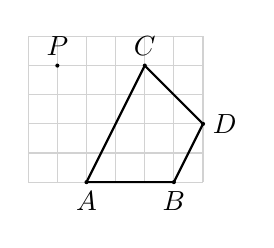
\begin{tikzpicture}[scale=.37]\draw[step=1,gray!35] (0,0) grid (6,5);\coordinate(A)at(2,0);\coordinate(B)at(5,0);\coordinate(C)at(4,4);\coordinate(D)at(6,2);\coordinate(P)at(1,4);\draw[thick](A)--(B)--(D)--(C)--cycle;\foreach \q/\lab/\pos in {A/A/below,B/B/below,C/C/above,D/D/right,P/P/above}{\fill(\q)circle(2pt)node[\pos]{$\lab$};}\end{tikzpicture}
\BookFigure{figures/p037_s08-02.tex}
\end{BookAnswer}

\Needspace{8\baselineskip}

\pdfbookmark[2]{原书第38页}{orig-38}

\subsection*{原书第38页}

% p038_s01
\BookQuestion{二、1}
两个完全相同的三角形一定能拼成（\hspace{1.8em}）。\par
\noindent A. 梯形\par
\noindent B. 平行四边形\par
\noindent C. 长方形\par
\noindent D. 正方形\par
\begin{BookAnswer}
选B。把两个完全相同的三角形的一组对应边重合，其中一个转半周，可以拼成两组对边分别平行的四边形。因此一定能拼成平行四边形；长方形、正方形需要额外角度条件。
\end{BookAnswer}

% p038_s02
\BookQuestion{二、2}
广场花坛的形状是平行四边形，相邻两条边长分别是7米和6米，这个花坛的周长是多少米？（\hspace{1.8em}）\par
\noindent A. 13米\par
\noindent B. 14米\par
\noindent C. 12米\par
\noindent D. 26米\par
\begin{BookAnswer}
选D。平行四边形的两组对边分别相等，周长\((7+6)\times2=26\)米，选D。
\end{BookAnswer}

% p038_s03
\BookQuestion{二、3}
一个等腰直角三角形，其中一个底角是（\hspace{1.8em}）。\par
\noindent A. \(90^\circ\)\par
\noindent B. \(180^\circ\)\par
\noindent C. \(45^\circ\)\par
\noindent D. \(60^\circ\)\par
\begin{BookAnswer}
选C。等腰直角三角形的两个锐角相等，共\(180^\circ-90^\circ=90^\circ\)，每个\(90^\circ\div2=45^\circ\)。
\end{BookAnswer}

% p038_s04
\BookQuestion{二、4}
校门口的电动伸缩门，能自由拉伸开合，它是利用了平行四边形（\hspace{1.8em}）的特性设计的。\par
\noindent A. 稳定性\par
\noindent B. 易变形\par
\noindent C. 对称性\par
\noindent D. 牢固性\par
\BookFigure{figures/p038_s04-01.tex}
\begin{BookAnswer}
选B。平行四边形四条边长度不变时，角度仍可以变化，所以容易变形，适合伸缩门自由拉伸。
\end{BookAnswer}

% p038_s05
\BookQuestion{二、5}
下面各组数据，不能组成三角形的是（\hspace{1.8em}）。\par
\noindent A. 6厘米、6厘米、6厘米\par
\noindent B. 3分米、3分米、6分米\par
\noindent C. 9米、7米、8米\par
\noindent D. 12厘米、6厘米、10厘米\par
\begin{BookAnswer}
选B。三角形任意两边之和必须大于第三边。B中\(3+3=6\)，只能排成一条直线；其余各组的两短边之和都大于最长边。
\end{BookAnswer}

% p038_s06
\BookQuestion{二、6}
裁剪窗花时，把一张平行四边形红纸任意分成两个梯形，这两个梯形的（\hspace{1.8em}）一定相等。\par
\noindent A. 面积\par
\noindent B. 周长\par
\noindent C. 高\par
\noindent D. 上底与下底的和\par
\begin{BookAnswer}
选C。两个梯形的两条底分别落在原平行四边形的同一组平行边上。高是从一条底到另一条底的垂直线段，表示这两条平行线之间的距离；所以两个梯形的高相等。分割线、斜腰或看起来较短的边，都不能直接当作高。面积、周长、两底之和则不一定相等。
\end{BookAnswer}

% p038_s07
\BookQuestion{二、7}
一个三角形中，最小的角是\(46^\circ\)，这个三角形是（\hspace{1.8em}）。\par
\noindent A. 锐角三角形\par
\noindent B. 直角三角形\par
\noindent C. 钝角三角形\par
\noindent D. 无法确定\par
\begin{BookAnswer}
选A。最小角为\(46^\circ\)，其余两个角都不小于\(46^\circ\)。最大角至多\(180^\circ-46^\circ-46^\circ=88^\circ\)，三个角都小于\(90^\circ\)，一定是锐角三角形。
\end{BookAnswer}

% p038_s08
\BookQuestion{三、1}
判断：长方形是特殊的平行四边形，正方形是特殊的长方形。（\hspace{1.8em}）\par
\begin{BookAnswer}
判\(\checkmark\)。长方形的两组对边分别平行，属于平行四边形；正方形四个角都为直角，属于长方形。
\end{BookAnswer}

% p038_s09
\BookQuestion{三、2}
判断：梯形的高一定比它的腰短。（\hspace{1.8em}）\par
\begin{BookAnswer}
判\(\times\)。直角梯形中，与底边垂直的那条腰就等于高，是反例。因此不能说高“一定比腰短”。
\end{BookAnswer}

% p038_s10
\BookQuestion{三、3}
判断：从平行四边形的一个顶点可以向对边作一条高，所以平行四边形有4条高。（\hspace{1.8em}）\par
\begin{BookAnswer}
判\(\times\)。平行四边形的边上有无数个点，都可向对边作垂线段，因此高有无数条，不能只数从顶点画出的几条。对应同一条底，所有高的长度相等；“长度相等”不表示“只有一条”。
\end{BookAnswer}

% p038_s11
\BookQuestion{三、4}
判断：两个完全一样的梯形可以拼成一个平行四边形。（\hspace{1.8em}）\par
\begin{BookAnswer}
判\(\checkmark\)。将两个完全相同的梯形反向拼接，使对应的一条腰重合，可拼成平行四边形，所得两组对边分别平行。
\end{BookAnswer}

% p038_s12
\BookQuestion{三、5}
判断：剪下三角形的一个\(45^\circ\)角，剩下图形的内角和是\(135^\circ\)。（\hspace{1.8em}）\par
\begin{BookAnswer}
判\(\times\)。不能把\(180^\circ\)直接减去剪下的\(45^\circ\)。沿一条线截去一个顶角，剩余部分可能成为四边形，其内角和为\(360^\circ\)；若剪线经过另一个顶点，剩余仍可能是三角形，内角和仍为\(180^\circ\)。
\end{BookAnswer}

% p038_s13
\BookQuestion{三、6}
判断：三角形越大，内角和就越大。（\hspace{1.8em}）\par
\begin{BookAnswer}
判\(\times\)。所有三角形的内角和都是\(180^\circ\)。图形放大或缩小，角度不变。
\end{BookAnswer}

% p038_s14
\BookQuestion{三、7}
判断：有一组对边平行的图形一定是梯形。（\hspace{1.8em}）\par
\begin{BookAnswer}
判\(\times\)。平行四边形也有一组对边平行，不能因此叫梯形。梯形必须是“只有一组对边平行”的四边形。
\end{BookAnswer}

\Needspace{8\baselineskip}

\pdfbookmark[2]{原书第39页}{orig-39}

\subsection*{原书第39页}

% p039_s01
\BookQuestion{四、1（1）}
按要求，画一画。（每两个格点之间的距离为1厘米）（1）以图中线段为三角形的底边，画一个等腰三角形，并画出底边上的高。\par
\BookFigure{figures/p039_s01-01.tex}
\begin{BookAnswer}
先数格找到给定底边的中点；沿经过中点、与底边垂直的方向取顶点，连接顶点与底边两端，得到等腰三角形。用三角尺检验：一条直角边贴底边，另一条直角边经过顶点；画出顶点到垂足的线段，标直角和“高”。原图示例的高经过底边中点，两腰相等。顶点取在底边任一侧，只要满足上述条件，都可以。
\BookFigure{figures/p039_s01-02.tex}
\end{BookAnswer}

% p039_s02
\BookQuestion{四、1（2）}
按要求，画一画。（每两个格点之间的距离为1厘米）（2）画一个梯形，并把梯形分成一个平行四边形和一个三角形。\par
\BookFigure{figures/p039_s02-01.tex}
\begin{BookAnswer}
先画只有一组对边平行的梯形。从一条上底的端点，画一条与不相邻的腰平行的线段，交下底于一点，就能分出一个平行四边形和一个三角形。也可从另一上底端点作对应分割，得到另一种画法。
\BookFigure{figures/p039_s02-02.tex}
\end{BookAnswer}

% p039_s03
\BookQuestion{四、2（1）}
画一画，写一写。（1）利用直尺和圆规，画出以线段\(a\)为底边，线段\(b\)和线段\(c\)为边的三角形。（保留作图痕迹）\par
\BookFigure{figures/p039_s03-01.tex}
\begin{BookAnswer}
先作线段\(AB=a\)。圆规开口取\(b\)，针尖固定在\(A\)画弧；再把开口调为\(c\)，针尖固定在\(B\)，在底边同一侧画弧，两弧交于\(C\)。连接\(AC,BC\)。因为圆规分别保持\(b,c\)的长度，所以\(AC=b,BC=c\)，三条边符合要求。要保留交点附近的弧线，每次画弧时圆规开口不能松动。交点取在底边另一侧也可，得到的两个三角形互为轴对称。
\BookFigure{figures/p039_s03-02.tex}
\end{BookAnswer}

% p039_s04
\BookQuestion{四、2（2）}
（2）根据你画的三角形，请提出一个值得思考的数学问题。（不用解答）\par
\begin{BookAnswer}
问题示例：这个三角形按角分类，属于什么三角形？也可以问：以最长边为底，这条底边上的高在三角形内部还是外部？题目说“不用解答”，提出与所画图形有关的合理问题即可。
\end{BookAnswer}

% p039_s05
\BookQuestion{五、1}
我国古代很早就用方正图形做器物，讲究几何之美。手工课上，李明用一根铁丝先围成了边长9厘米的正方形，如果要用这块铁丝围成一个等边三角形，它的边长是多少厘米？（7分）\par
\begin{BookAnswer}
铁丝总长度不变，先按正方形每边9厘米乘4条边列式，再按等边三角形的3条边平均分。计算时先除以3，再乘4，更便于口算。\[\begin{aligned}&9\times4\div3\\={}&9\div3\times4\\={}&3\times4\\={}&12\text{(厘米)}\end{aligned}\]答：等边三角形的边长是12厘米。\par 另一数量理解：每条原边平均分成3小份，共12小份，每条新边取4小份，直接得到\(9\div3\times4\)。它与上面的简算式一致，不重复列第二遍脱式。
\end{BookAnswer}

\Needspace{8\baselineskip}

\pdfbookmark[2]{原书第40页}{orig-40}

\subsection*{原书第40页}

% p040_s01
\BookQuestion{五、2}
在下面的三角形中，已知\(\angle1=75^\circ\)，\allowbreak{}\(\angle2=60^\circ\)，你能求出\(\angle3\)和\(\angle4\)的度数吗？想一想：\(\angle4\)、\(\angle1\)、\(\angle2\)有什么关系？（7分）\par
\BookFigure{figures/p040_s01-01.tex}
\begin{BookAnswer}
方法一：先用三角形内角和求\(\angle3\)，再用平角求\(\angle4\)。\[\begin{aligned}\angle3&=180^\circ-75^\circ-60^\circ\\&=105^\circ-60^\circ\\&=45^\circ,\\\angle4&=180^\circ-45^\circ\\&=135^\circ.\end{aligned}\]\par 方法二：比较三角形的内角和与底边上的平角，去掉共同的\(\angle3\)，便知\(\angle4\)等于另外两个内角的和。\[\begin{aligned}\angle4&=75^\circ+60^\circ\\&=135^\circ,\\\angle3&=180^\circ-135^\circ\\&=45^\circ.\end{aligned}\]\par 答：\(\angle3=45^\circ,\angle4=135^\circ\)，关系为\(\angle4=\angle1+\angle2\)。这里从已学的内角和、平角推得关系，不要求背诵新的定理名称。
\end{BookAnswer}

% p040_s02
\BookQuestion{五、3}
一根长11厘米的细铁丝，先把它分成三段，再首尾相接围成一个三角形，应该怎样分？小优在2厘米处剪了一刀，再在哪个刻度剪一刀就能围成一个三角形？请你先在图中标出剪的位置，再把想法写出来。（边长为整厘米数）（8分）\par
\BookFigure{figures/p040_s02-01.tex}
\begin{BookAnswer}
方法一：先确定两条余边，再还原剪切位置。第一刀已剪下2厘米，余下两条边的总长是：\[\begin{aligned}&11-2\\={}&9\text{(厘米)}\end{aligned}\]另外两边为整厘米数，和为9、差小于2，只能是4厘米和5厘米。第二刀的位置有两种：\[\begin{aligned}&2+4\\={}&6\text{(厘米)}\end{aligned}\]\[\begin{aligned}&2+5\\={}&7\text{(厘米)}\end{aligned}\]答：可以在6厘米处或7厘米处剪。两种剪法的三边都是2、4、5厘米，满足\(2+4>5\)。\par 方法二：逐一检查整厘米剪切位置。第二刀须落在余下的9厘米部分，可试3至10厘米处。\[\begin{array}{c|c|c}\text{剪切位置}&\text{三边长}&\text{能否围成}\\\hline3&2,1,8&\times\\4&2,2,7&\times\\5&2,3,6&\times\\6&2,4,5&\checkmark\\7&2,5,4&\checkmark\\8&2,6,3&\times\\9&2,7,2&\times\\10&2,8,1&\times\end{array}\]只需检查两条较短边之和是否大于最长边。答：仍为6厘米处或7厘米处；图中两处短线表示备选位置，实际只再剪一处。
\par\smallskip\Needspace{4\baselineskip}\begingroup\small\setlength{\tabcolsep}{3pt}
\noindent\begin{tabularx}{\linewidth}{|*{3}{>{\centering\arraybackslash}X|}}\hline
第二刀刻度（厘米） & 三边长（厘米） & 能否围成\\\hline
\textcolor{answerred}{3} & \textcolor{answerred}{2、1、8} & \textcolor{answerred}{不能}\\\hline
\textcolor{answerred}{4} & \textcolor{answerred}{2、2、7} & \textcolor{answerred}{不能}\\\hline
\textcolor{answerred}{5} & \textcolor{answerred}{2、3、6} & \textcolor{answerred}{不能}\\\hline
\textcolor{answerred}{6} & \textcolor{answerred}{2、4、5} & \textcolor{answerred}{能}\\\hline
\textcolor{answerred}{7} & \textcolor{answerred}{2、5、4} & \textcolor{answerred}{能}\\\hline
\textcolor{answerred}{8} & \textcolor{answerred}{2、6、3} & \textcolor{answerred}{不能}\\\hline
\textcolor{answerred}{9} & \textcolor{answerred}{2、7、2} & \textcolor{answerred}{不能}\\\hline
\textcolor{answerred}{10} & \textcolor{answerred}{2、8、1} & \textcolor{answerred}{不能}\\\hline
\end{tabularx}\par
\endgroup\smallskip
\BookFigure{figures/p040_s02-02.tex}
\end{BookAnswer}

% p040_s03
\BookQuestion{六、思考题}
科技小组制作AI扫地机器人防撞外壳，取用一块直角梯形塑料板，沿一条线段切割，分成一个平行四边形和一个直角三角形。已知梯形下底比上底长3厘米，梯形两条腰长度之和为10厘米。若给分出的直角三角形围一圈防撞条，你能算出这个直角三角形的周长吗？（4分）\par
\BookFigure{figures/p040_s03-01.tex}
\begin{BookAnswer}
右侧切出的直角三角形，一条直角边长等于梯形两底之差3厘米。另外两条边分别与梯形的两腰等长（利用平行四边形对边相等），其和为10厘米。\[\begin{aligned}&10+3\\&=13\text{(厘米)}\end{aligned}\]\par 答：防撞条一圈的长度，即直角三角形的周长，是13厘米。\par 也可从周长转移来理解：原来梯形两腰的总长10厘米都保留到三角形中，再增加两底之差3厘米。
\end{BookAnswer}
